% Drawing 154/01-15 -- folder 154, batch 01, archive page 11 (PDF page 12).
% Transcription: figure, à gauche : un faisceau de droites orange issues d'un point $s$, coupant un segment jaune en quatre points marqués, le premier noté $r$ et le dernier $t$
% Kind: pencil of lines through a point, cut by a segment. Method 2 (schematic redraw from the facsimile). Status: ok.
% Notes: Four orange lines through s, each through one of the four black points of the yellow segment (computed: s once, the points on the segment); a pencil line along the second orange line and two pencil strokes inside the triangle; labels r, s, t. The transcription's note counts three points between r and t: on the page there are four points in all, r written by the first and t by the last. The word beside the figure (read « critère-rive ») belongs to the text and is not drawn. Redrawn 2026-11-12 (issue 128): to check again.
% Coordinates: 1 unit = 1 mm = 1/100 of the crop width (bbox in page fractions: [0.19, 0.17, 0.32, 0.225]).
% Redrawn by Claude (claude-fable-5-2), issue #128, 2026-11-12; not checked by a human; not compiled (no TeX in the session).
% Rights: reproduces part of the work -- behind RENDER_TRANSCRIPTS, never published by itself.
\documentclass[tikz,border=3pt]{standalone}
\usepackage{amsmath,amssymb}
\usetikzlibrary{patterns,arrows.meta}
\tikzset{Or/.style={orange!90!black}, Ye/.style={yellow!80!orange}, pencil/.style={black!45}, struck/.style={black!35}, mpt/.style={circle,draw,inner sep=1.3pt}, pt/.style={circle,fill,inner sep=0.9pt}, opt/.style={circle,draw,fill=white,inner sep=1.1pt}}
\begin{document}
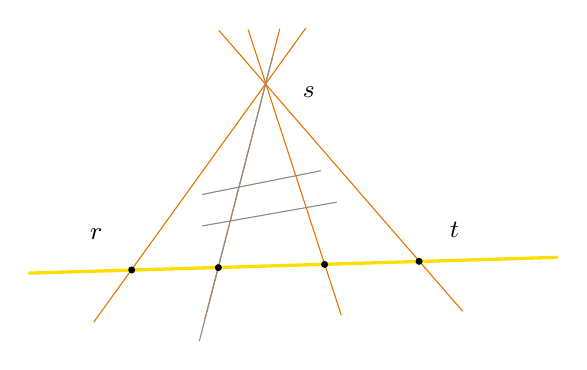
\begin{tikzpicture}[x=1mm,y=1mm,line cap=round,line join=round,font=\scriptsize]
\draw[Ye,very thick] (23,-51) -- (90,-49);
\draw[Or] (31.2,-57.2) -- (58.1,-19.9);
\draw[Or] (45.3,-56.8) -- (54.8,-20);
\draw[Or] (62.6,-56.3) -- (50.8,-20.1);
\draw[Or] (78,-55.8) -- (47.1,-20.2);
\draw[pencil] (44.6,-59.6) -- (53.9,-23.5);
\draw[pencil] (45,-41) -- (60,-38);
\draw[pencil] (45,-45) -- (62,-42);
\node[pt] at (36,-50.6) {};
\node[pt] at (47,-50.3) {};
\node[pt] at (60.5,-49.9) {};
\node[pt] at (72.5,-49.5) {};
\node[inner sep=1pt] at (31.5,-46) {\small $r$};
\node[inner sep=1pt] at (77,-45.5) {\small $t$};
\node[inner sep=1pt] at (58.5,-28) {\small $s$};
\end{tikzpicture}
\end{document}
